\documentclass[11pt]{article}

\usepackage{latexsym}
\usepackage{amssymb}
\usepackage{amsthm}
\usepackage{enumerate}
\usepackage{amsmath}
\usepackage{cancel}
\usepackage{graphicx}
\numberwithin{equation}{section}
\numberwithin{figure}{section}
\numberwithin{table}{section}

\setlength{\evensidemargin}{.25in}
\setlength{\oddsidemargin}{-.25in}
\setlength{\topmargin}{-.75in}
\setlength{\textwidth}{6.5in}
\setlength{\textheight}{9.5in}
\newcommand{\due}{February 10th, 2010}
\newcommand{\HWnum}{2}
\newcommand{\grad}{\bold\nabla}
\newcommand{\vecE}{\vec{E}}
\newcommand{\scrptR}{\vec{\mathfrak{R}}}
\newcommand{\kapa}{\frac{1}{4\pi\epsilon_0}}

\begin{document}
\begin{titlepage}
\setlength{\topmargin}{1.5in}
\begin{center}
\Huge{Physics 3320} \\
\LARGE{Principles of Electricity and Magnetism II} \\
\Large{Professor Ana Maria Rey} \\[1cm]

\huge{Homework \#\HWnum}\\[0.5cm]

\large{Joe Becker} \\
\large{SID: 810-07-1484} \\
\large{\due} 

\end{center}

\end{titlepage}



\section{Introduction}
The ability to separate signal from background noise is vitally important in experimental physics. Often we need to filter out background frequencies from our signal. Low pass, high pass, and band pass filters are a common way to for physicists to expose a signal. 

This experiment is designed to demonstrate the response of four simple circuits: the voltage divider, low pass, high pass, and band pass filters to different frequencies. We will compare the changes to the attenuation ($V_{in}/V_{out}$) to increasing frequencies of a sinusoidal input voltage. We will also measure the exponential rise-time, $t_R$, of the integrator circuit (high pass filter) and the decay-time, $t_D$, of the differentiator circuit (low pass filter) when we input a square wave. In the next section we will cover the expected responses of each of these circuits.

\section{Theory}
The four circuits we analyze each have a different response to a changing input frequency. We well go over each on individually. For all four circuits we use the relation
\begin{equation}
|T| = \frac{V_{out}}{V_{in}}
\label{atten}
\end{equation}
as the definition of attenuation. Where we write the gain of the attenuation using
\begin{equation}
dB = 20\log|T|
\label{gain}
\end{equation}
Note that $dB$ is a dimensionless unit. 

\subsection{The Voltage divider}
The voltage divider circuit does just what its name implies. As we can see from the schematic of this circuit as seen in figure \ref{FigVoltDiv}
\begin{figure}[h]
\centering
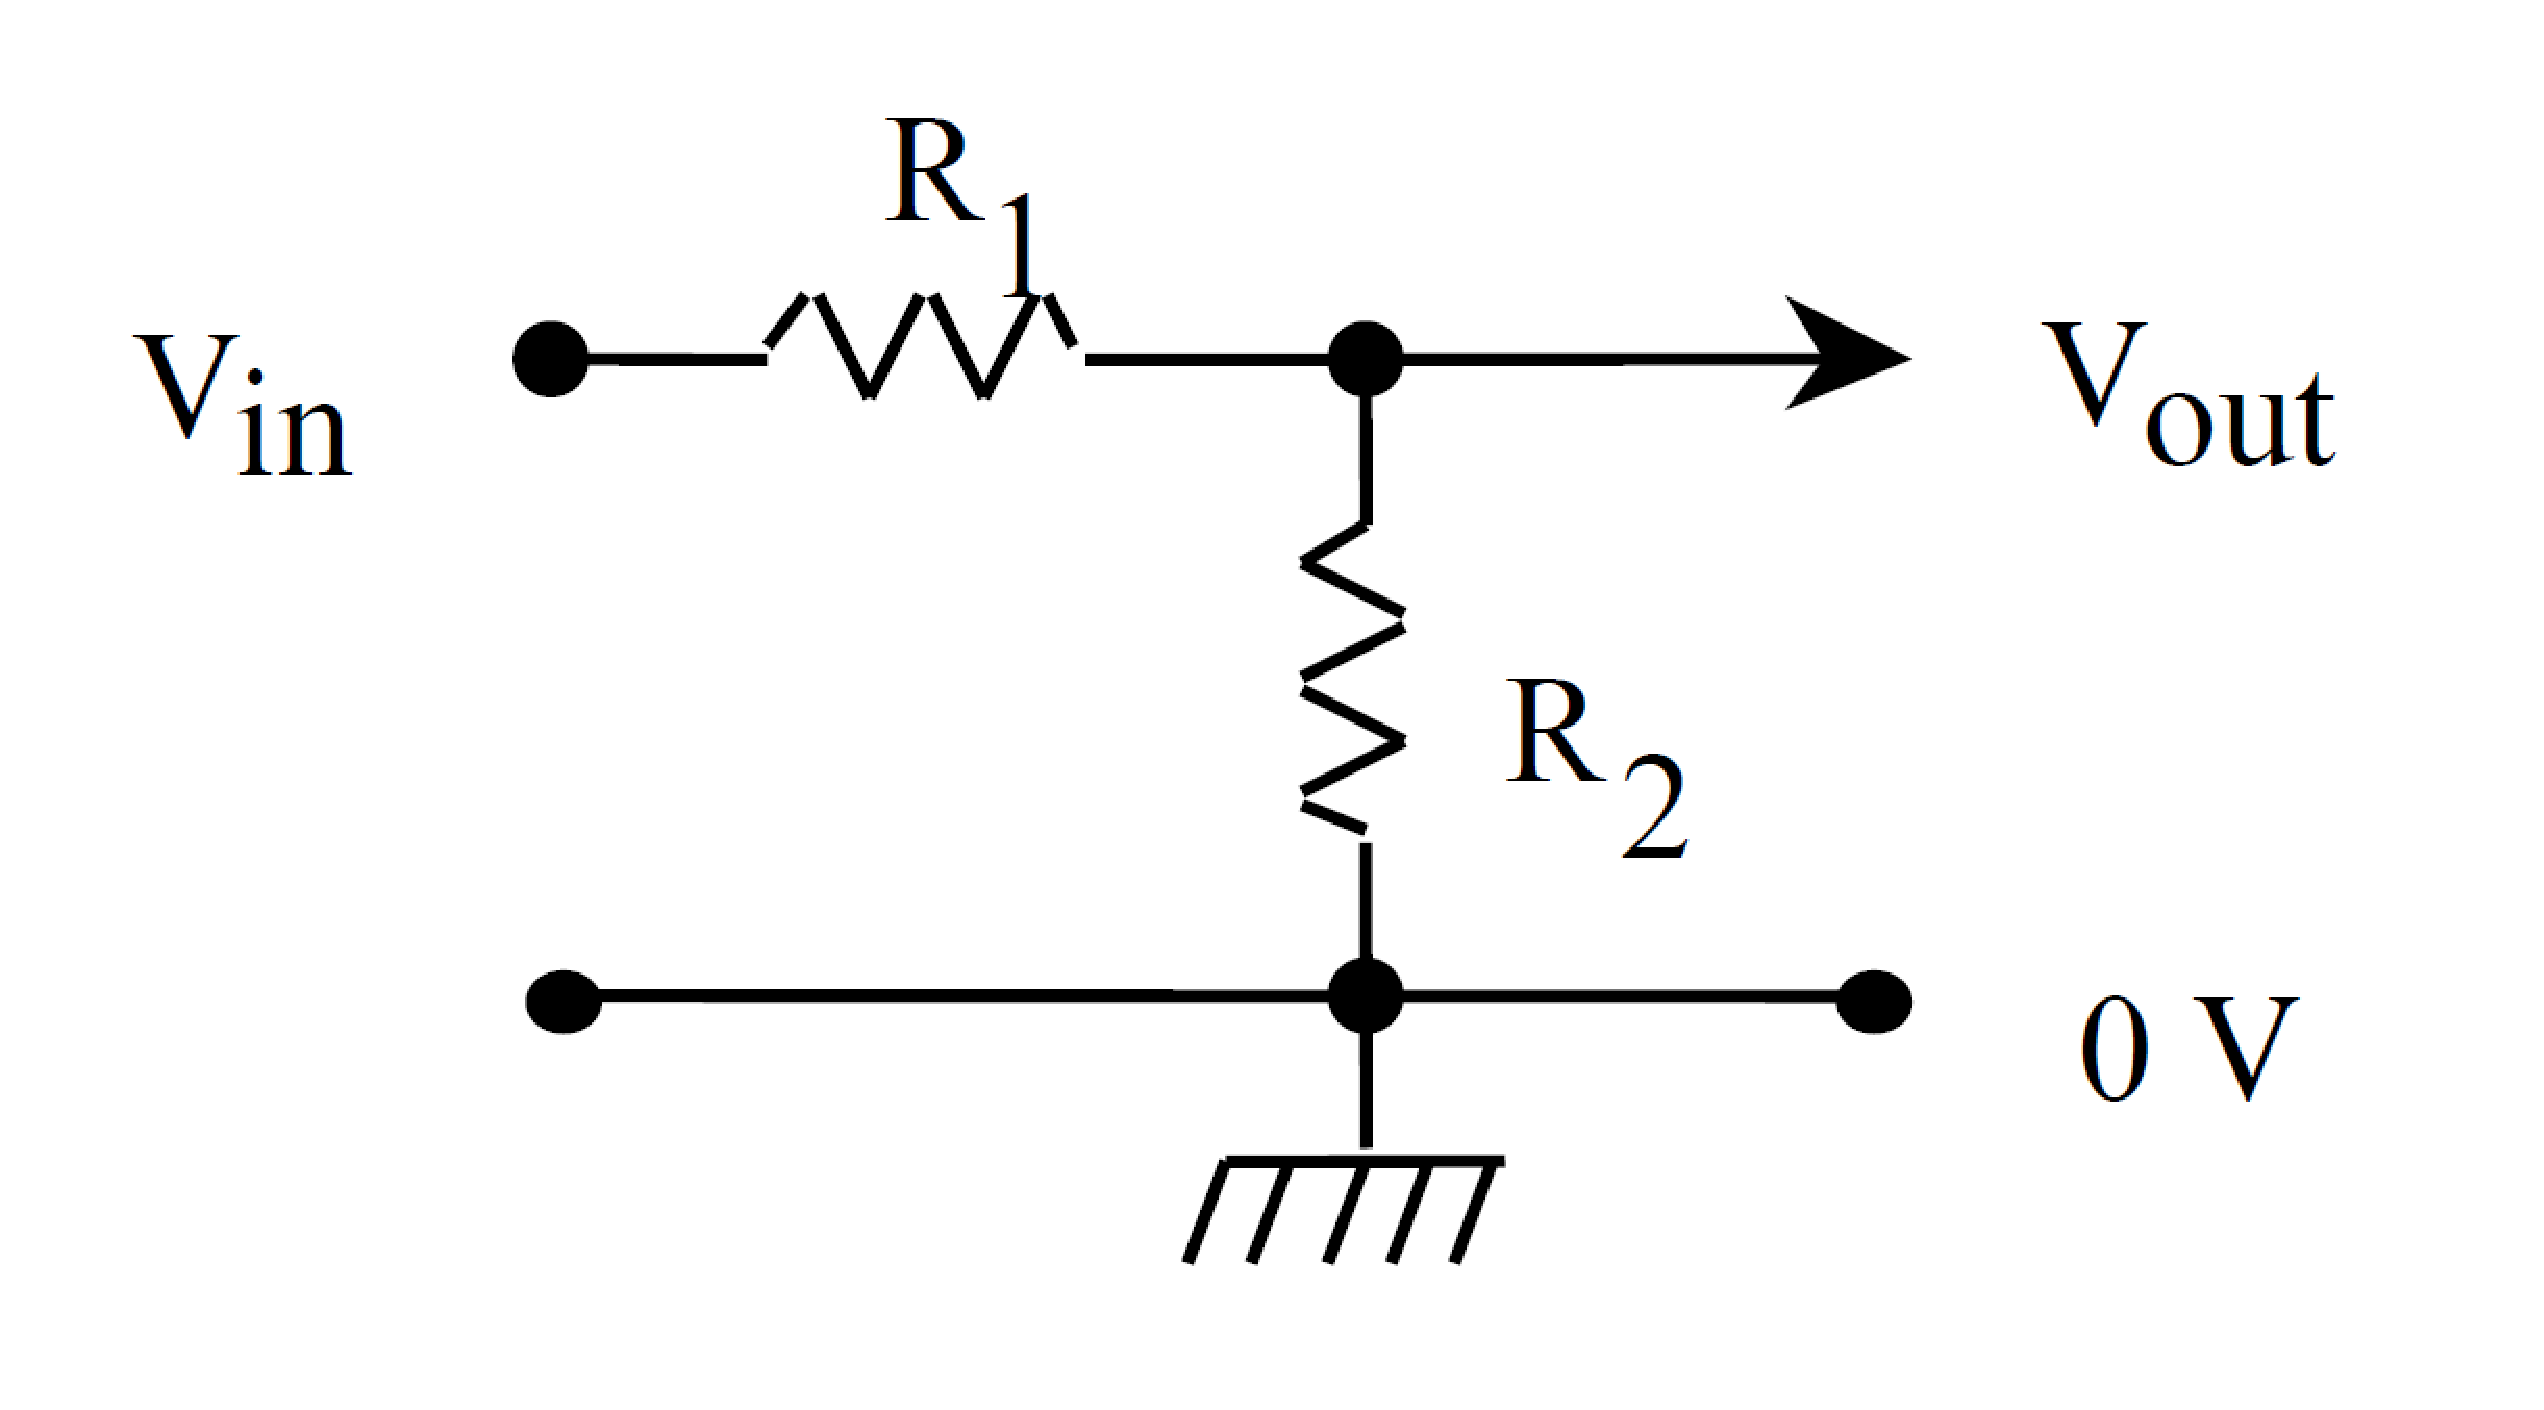
\includegraphics[scale=0.20]{Volt.Div.eps}
\caption{\textit{The schematic for the voltage divider circuit}}
\label{FigVoltDiv}
\end{figure}
the input voltage, $V_{in}$, is divided by a fixed ratio such that
\begin{equation}
V_{out} = \frac{R_2}{R_1+R_2}V_{in}
\label{VoltDiv.InvOut}
\end{equation}
Now we see that if we divide out the $V_{in}$ in equation \ref{VoltDiv.InvOut} we see that the attenuation, $|T|$, of this circuit is given by
$$\frac{V_{out}}{V_{in}} = |T| = \frac{R_2}{R_1+R_2}$$
This equation implies the fact that the attenuation of the voltage divider is not dependent on the input frequency. So we expect that the attenuation of the voltage divider will not change when we change the frequency of the input voltage and a Bode plot of the attenuation versus frequency will be a flat line with the value of $R_1/(R_1+R_2)$. We also see that this circuit has no exponential rise-time or decay time as it only scales the voltage. 

\subsection{The Low-Pass Filter}
The low-pass filter is a RC circuit that, as its name suggests, filters out high frequencies of the input sinusoidal voltages. We can see the schematic for this circuit in figure \ref{FigLowPass}.
\begin{figure}[h]
\centering
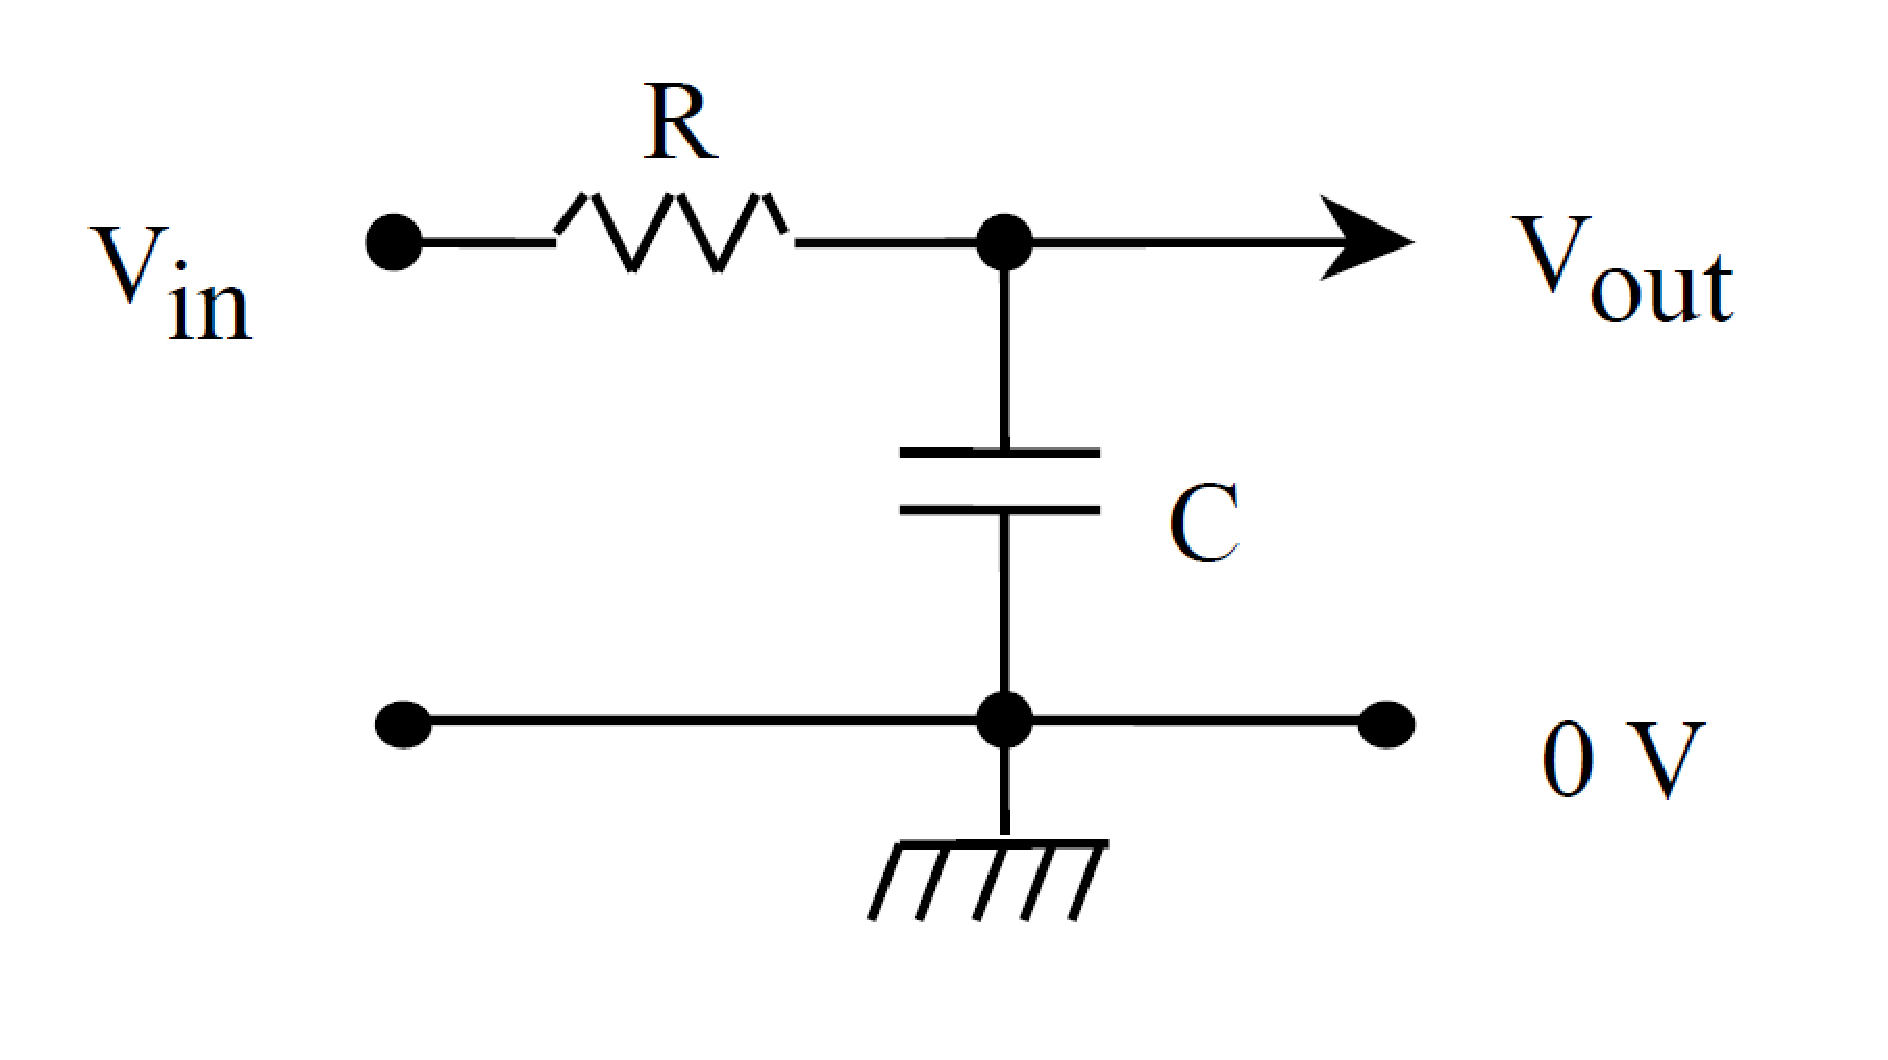
\includegraphics[scale=0.20]{LowPass.eps}
\caption{\textit{The schematic for the low-pass filter}}
\label{FigLowPass}
\end{figure}
We see that the attenuation is given by 
\begin{equation}
|T|^2 = \frac{1}{1+(\omega RC)^2}
\label{AttenLowPass}
\end{equation}
Where $\omega$ is the angular frequency and is related to the normal frequency by $\omega = 2\pi f$. It is important to note that the frequency at which equation \ref{AttenLowPass} halves, or the $3\ dB$ point, is determined by
\begin{equation}
f_c = \frac{1}{2\pi RC}
\label{ResFreq}
\end{equation}
This point is an important point, because for frequencies below $f_c$ the attenuation is near one. And for frequencies above $f_c$ the attenuation is near zero. This fact leads to Bode plots that look like figure \ref{BodeLowPass}
\begin{figure}[h]
\centering
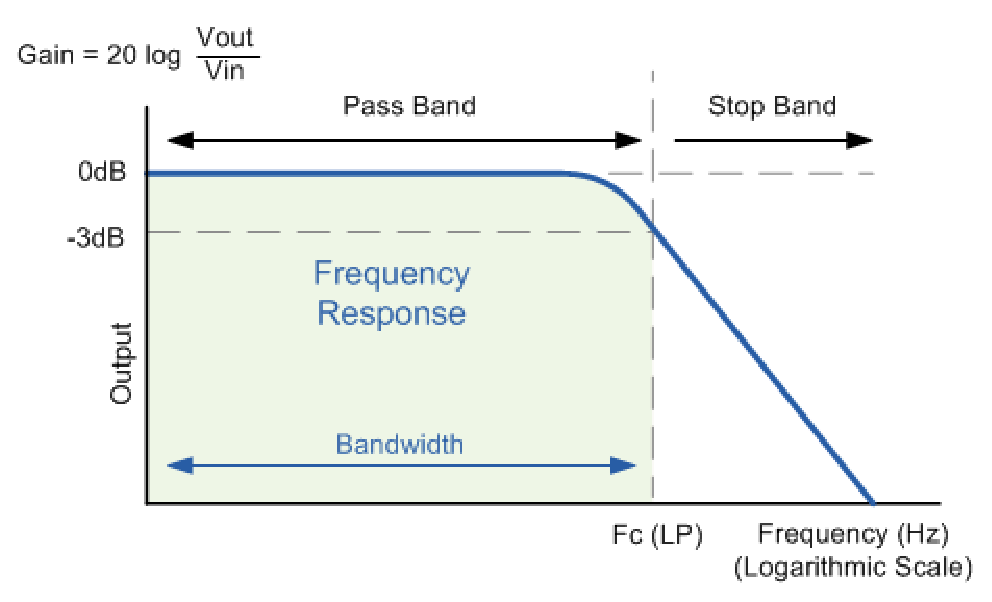
\includegraphics[scale=0.65]{BodeLowPass.eps}
\caption{\textit{The Bode plot for the low-pass filter. Note the $f_c$ point is the point at which the curve is changing the most.}}
\label{BodeLowPass}
\end{figure}

This circuit is also referred to as an \emph{integrator circuit} when the input voltage is a square wave. The output voltage rises exponentially to the top of the square wave. We call the quantity $t_R$ the exponential time rise of the integrator. The exponential time rise is calculated from
\begin{equation}
t_R = RC
\label{TimeRise}
\end{equation}
We can also find $t_R$ empirically from the output voltage. $t_R$ is the time it takes to get to $67\%$ of the maximum of $V_{out}$. This point can be seen on figure \ref{Integ}.
\begin{figure}[h]
\centering
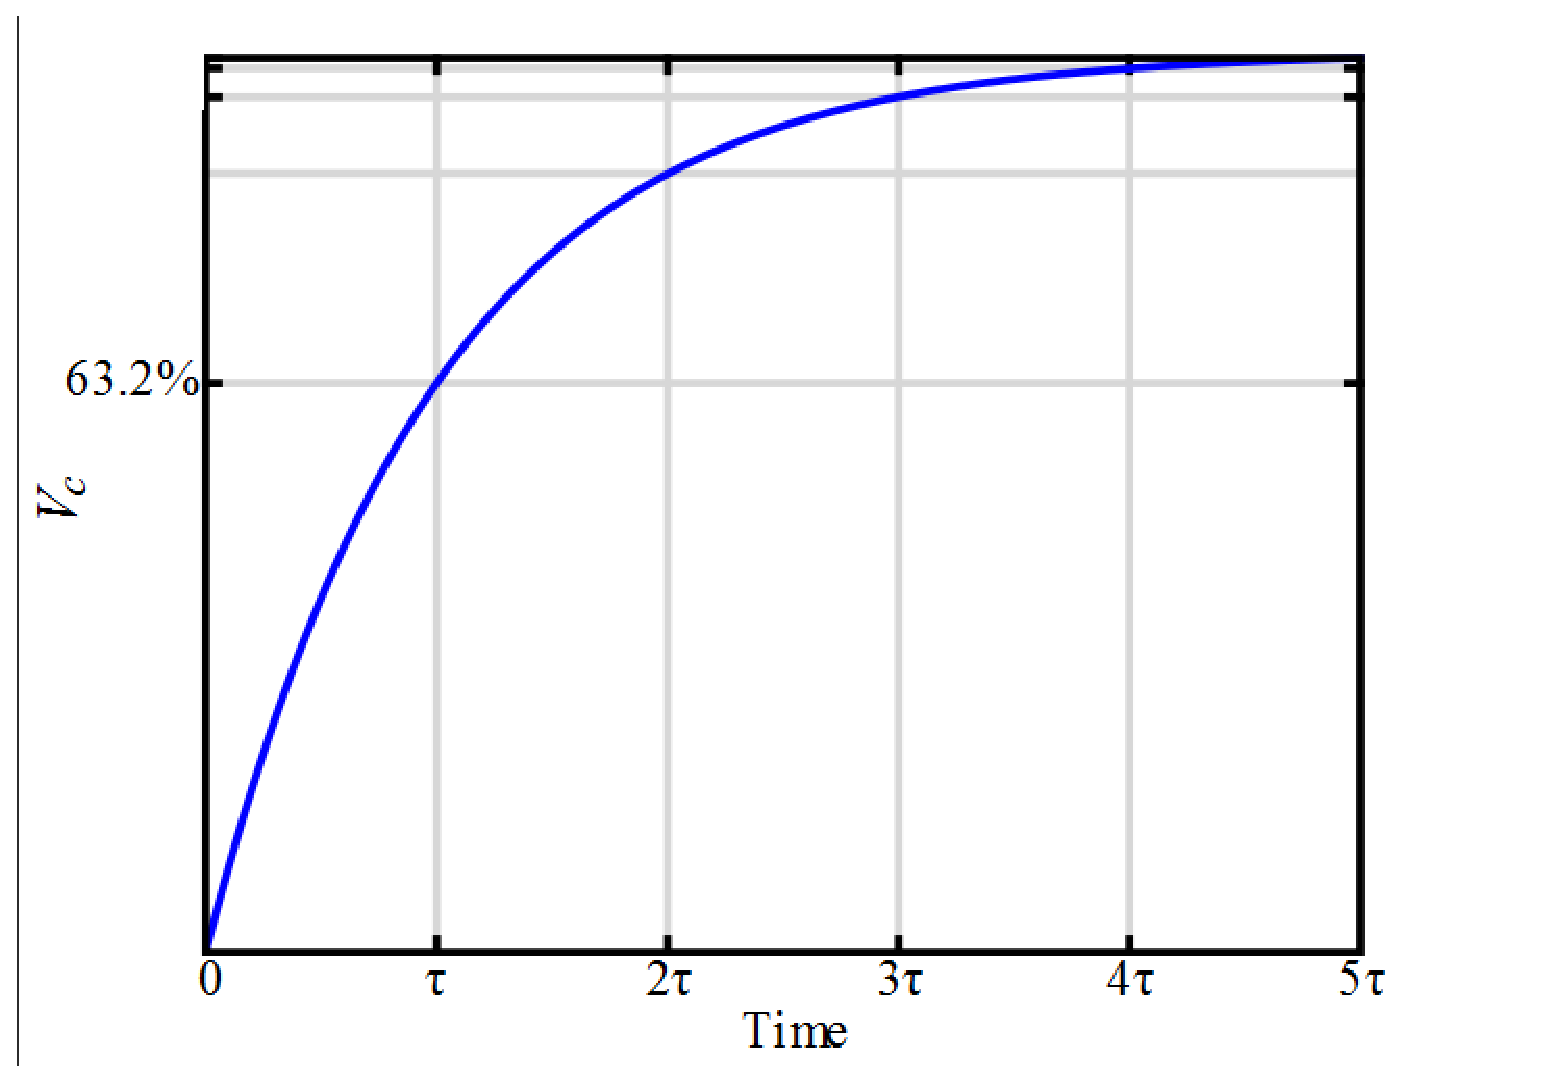
\includegraphics[scale=0.40]{Integ.eps}
\caption{\textit{The integrator circuit's response. Note the $67\%$ point verses the exponential time rise $t_R$.}}
\label{Integ}
\end{figure}

\subsection{The High-Pass Filter}
Like the low-pass filter, the high-pass filter is a simple RC circuit described by figure \ref{FigHighPass}. The high-pass filter acts in the opposite way as the low-pass filter. Higher frequencies are let through and lower frequencies are filtered out.
\begin{figure}[h]
\centering
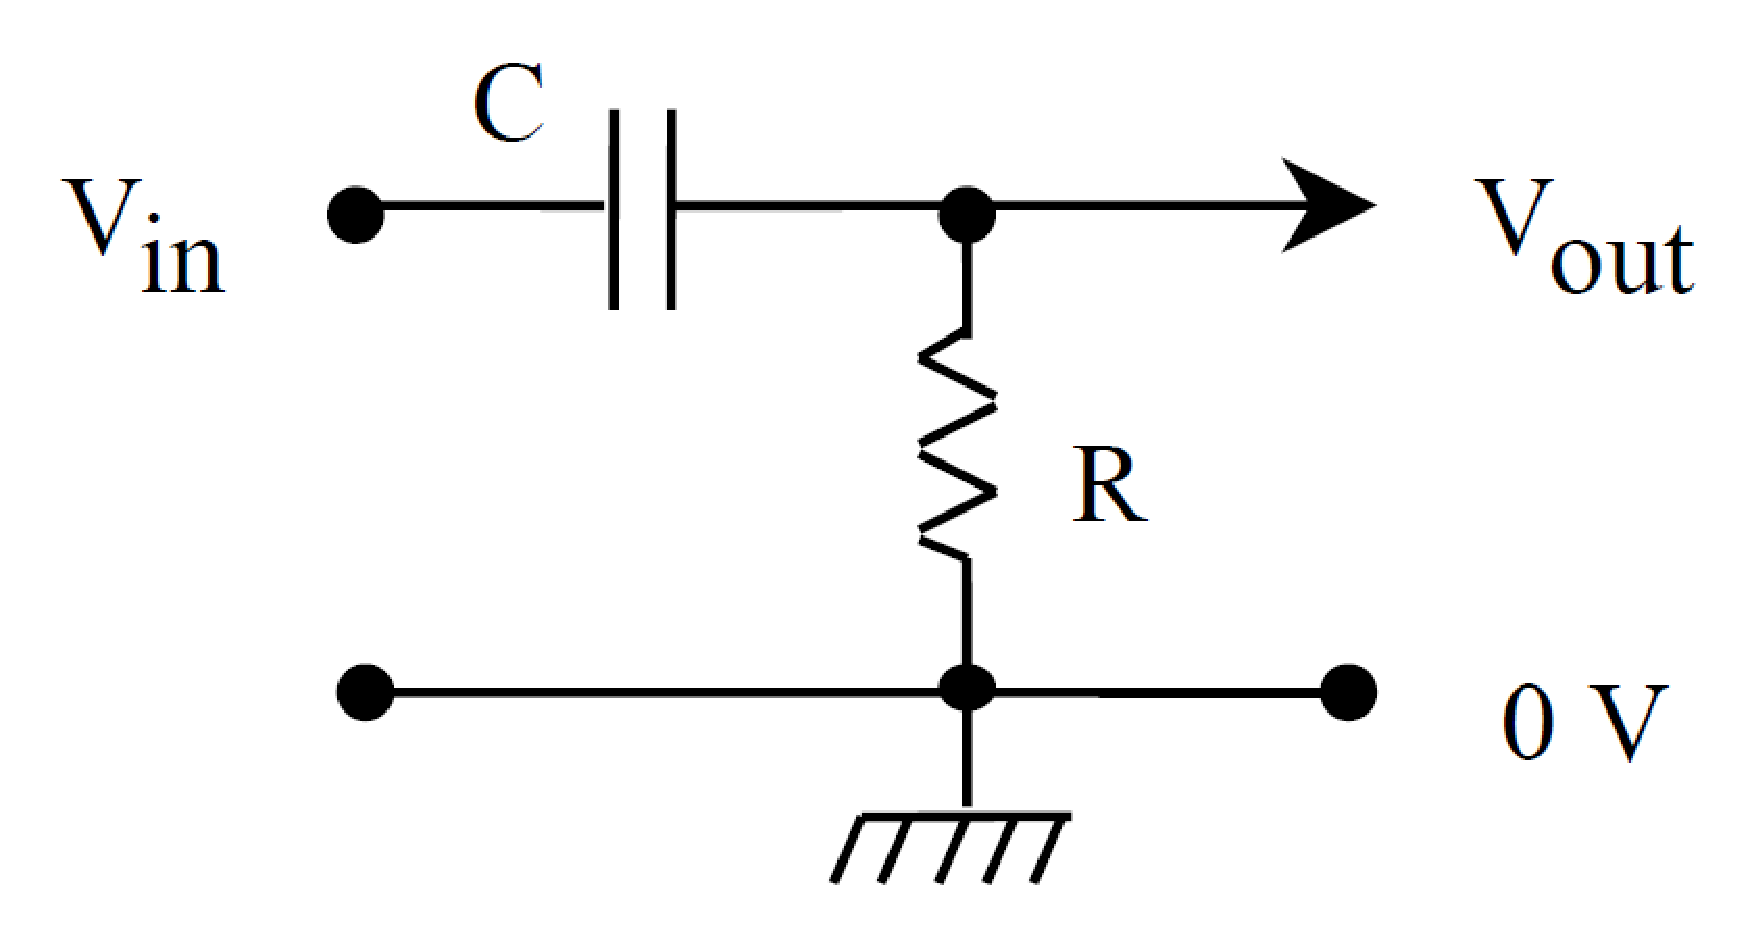
\includegraphics[scale=0.20]{HighPass.eps}
\caption{\textit{The schematic for the high-pass filter}}
\label{FigHighPass}
\end{figure}
We can say that the attenuation of the circuit is given by
\begin{equation}
|T|^2 = \frac{(R\omega C)^2}{1+(R\omega C)^2}
\label{AttenHighPass}
\end{equation}
We see that the $3\ dB$ point of this circuit is the same as equation \ref{ResFreq}. The key difference between this circuit and the low-pass circuit is that frequencies above $f_c$ the transfer function is near zero and for frequencies above the attenuation. So we see we get a Bode plot represented by figure \ref{BodeHighPass}.
\begin{figure}[h]
\centering
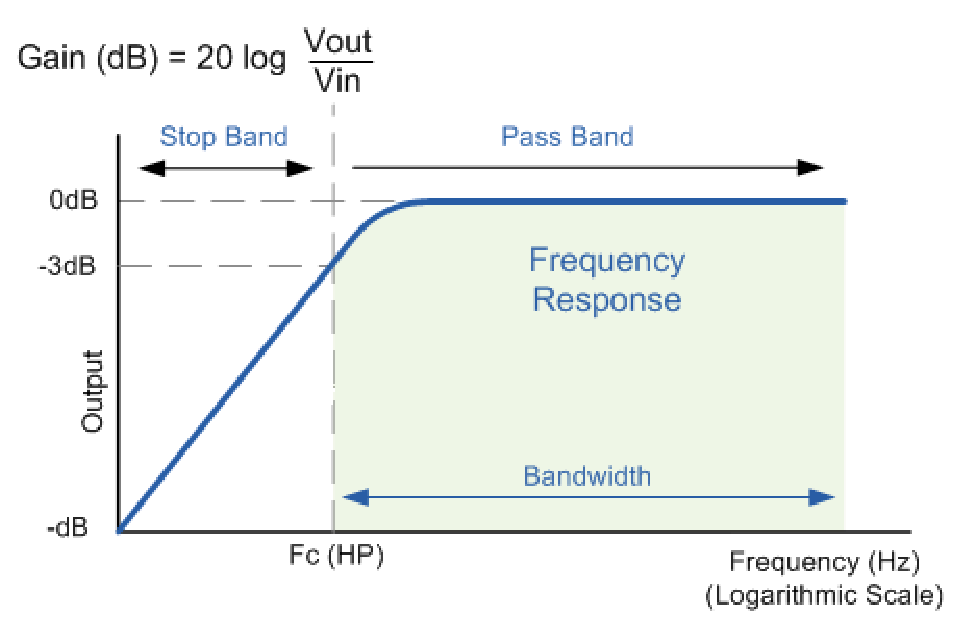
\includegraphics[scale=0.65]{BodeHighPass.eps}
\caption{\textit{The Bode plot for the high-pass filter. Note the $f_c$ point is the point at which the curve changes.}}
\label{BodeHighPass}
\end{figure}

The high-pass circuit is also referred to as a \emph{differentiator circuit} when the input voltage is a square wave. The output voltage decays exponentially down from the pulse of the square wave. The rate of decay of the voltage is described by the time-decay $t_D$ which is given by
\begin{equation}
t_D = RC
\label{TimeDecay}
\end{equation} The time-decay is also the time it takes for the voltage to fall $67\%$ of the maximum voltage. This point is shown in figure \ref{Differ}.
\begin{figure}[h]
\centering
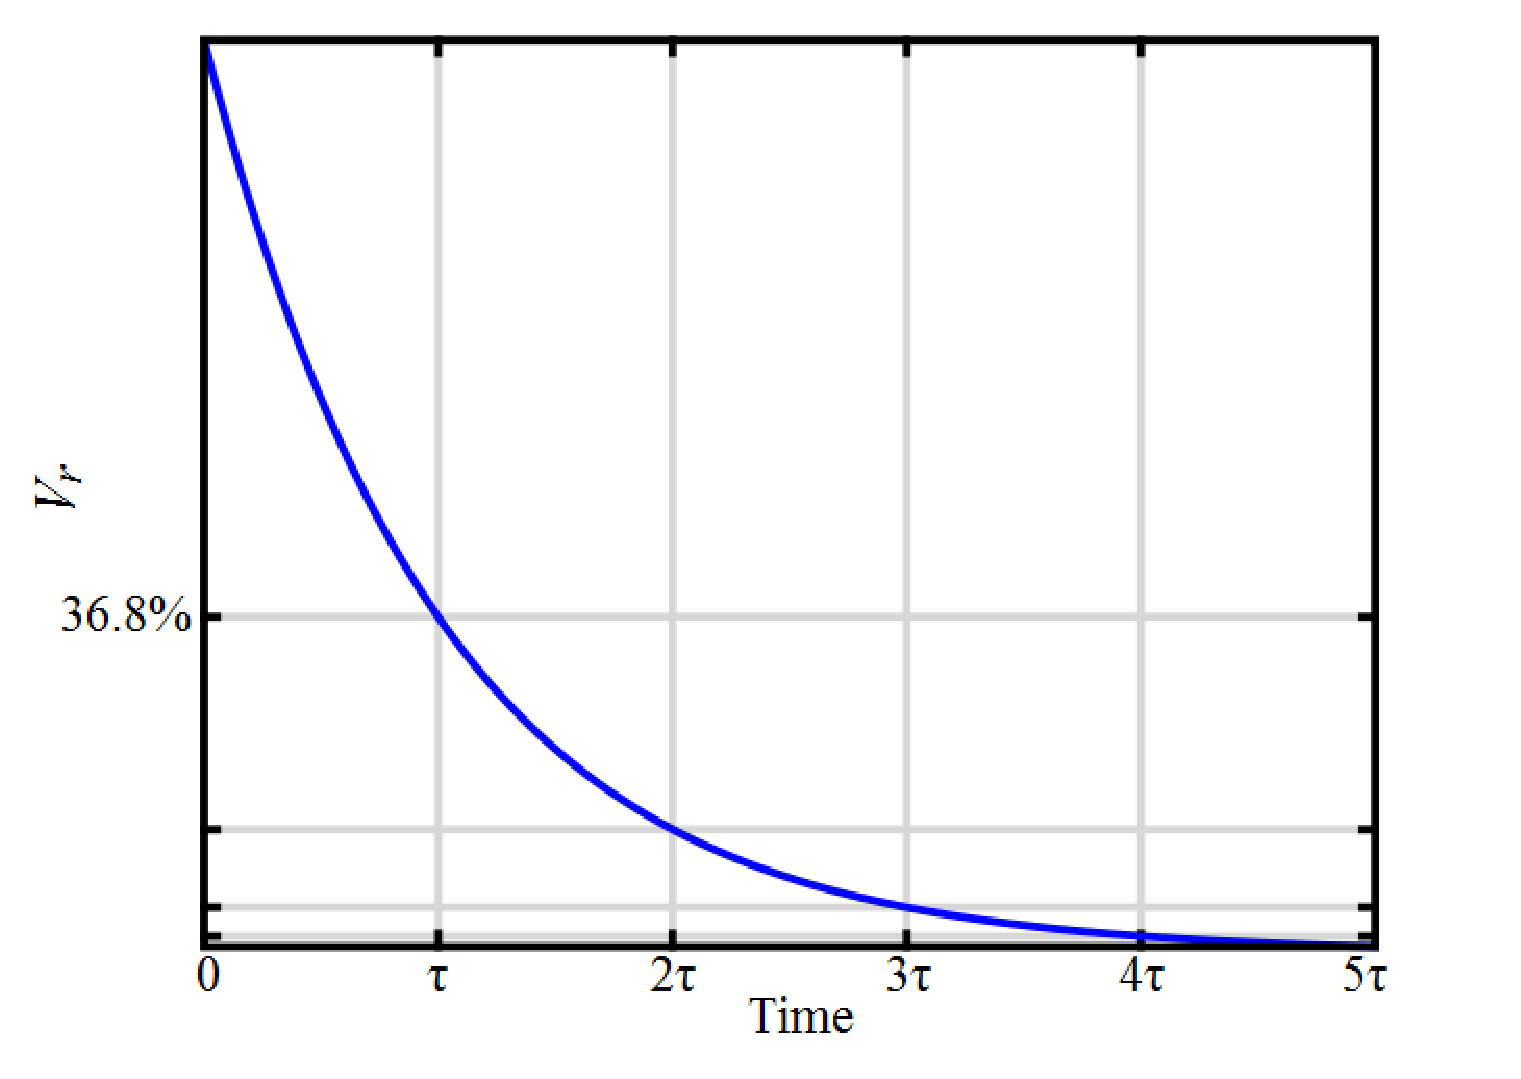
\includegraphics[scale=0.40]{Differ.eps}
\caption{\textit{The differentiator's response to a pulse of the square wave.}}
\label{Differ}
\end{figure}

\subsection{The Band-Pass Filter}
The band-pass filter is a simple LRC circuit which is described by figure \ref{FigBandPass}. A band-pass filter filters out frequencies except for those near the resonant frequency, $f_c$. Where $f_c$ is derived from the transfer function

\begin{figure}[h]
\centering
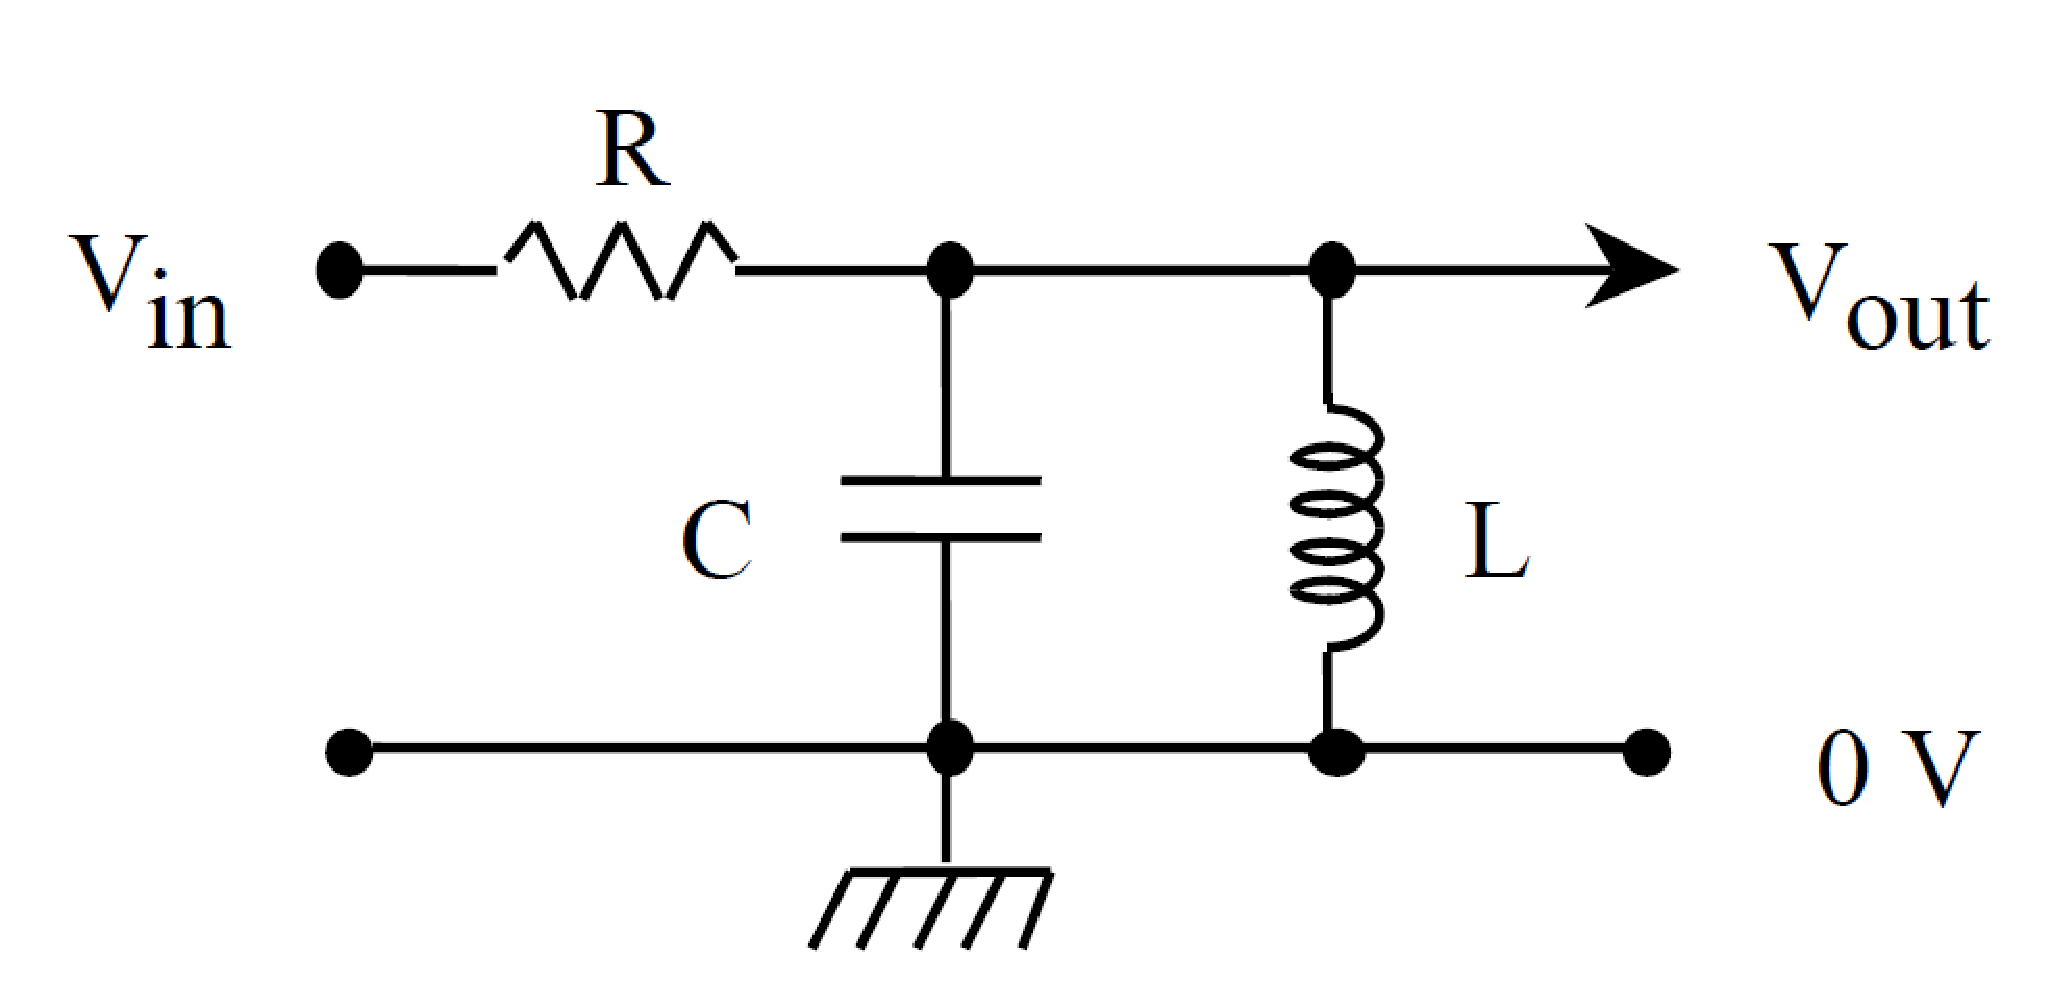
\includegraphics[scale=0.20]{BandPass.eps}
\caption{\textit{The schematic for the band-pass filter}}
\label{FigBandPass}
\end{figure}

\begin{equation}
T = \frac{1}{j(RC/L)(\omega L - 1/\omega C)+1}
\label{TranBandPass}
\end{equation}
We see that when equation \ref{TranBandPass} is at a maximum, the angular frequency is given by
$$\omega_0 = \frac{1}{\sqrt{LC}}$$ 
or using the relation $\omega_0 = 2\pi f_0$ so
\begin{equation}
f_0 = \frac{1}{2\pi\sqrt{LC}}
\label{BandPassResFreq}
\end{equation}
Now we see the point where the transfer function is at a maximum, but the width of the band that gets makes it through the filter is given by the quality factor, $Q$. We can find $Q$ from
\begin{equation}
Q = \omega_0 RC
\label{QualFact}
\end{equation}
The quality factor is also related to the width of the Bode plot (see figure \ref{BodeBandPass}) of the band-pass filter. We define a quantity $\Delta f$ as the bandwidth. Where $\Delta f$ is the width of the Bode plot $3\ dB$ down from the resonant frequency, $f_0$. $Q$ is related to $\Delta f$ and $f_0$ through the equation
\begin{equation}
Q = \frac{f_0}{\Delta f}
\label{QualDF}
\end{equation}
So the larger the $Q$ factor the more narrow the bandwidth.

\begin{figure}[h]
\centering
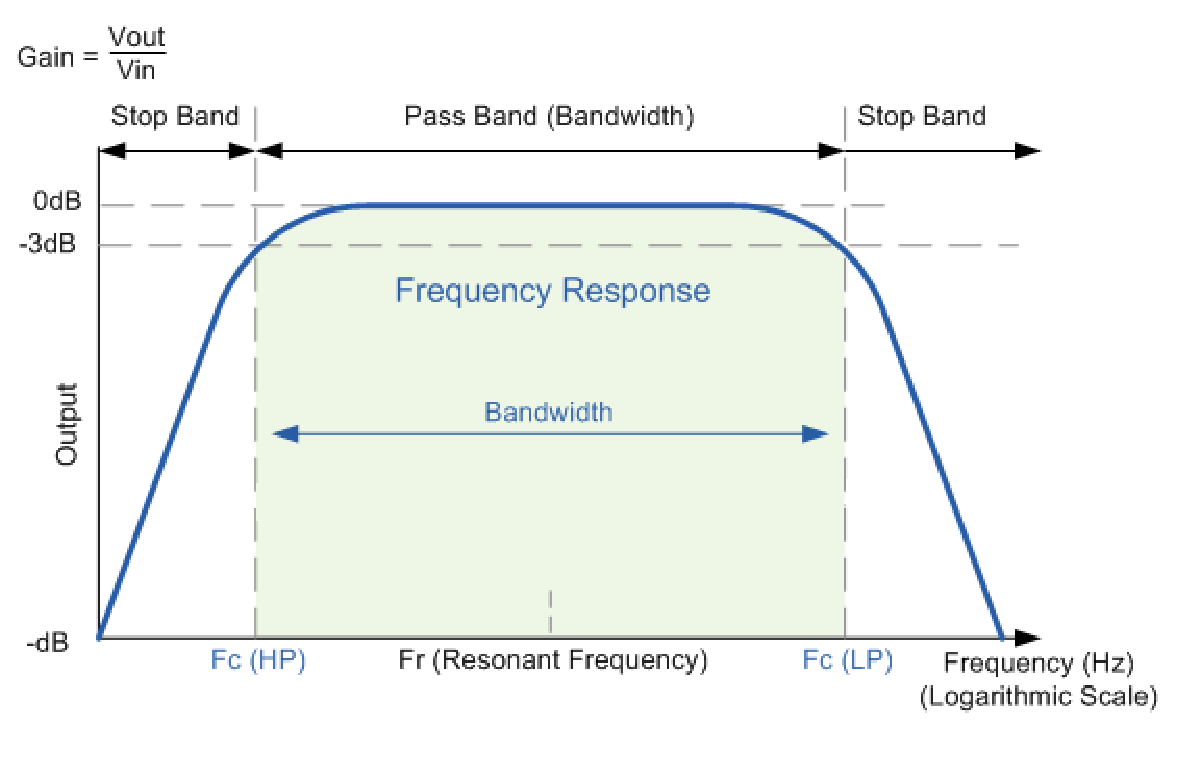
\includegraphics[scale=0.65]{BodeBandPass.eps}
\caption{\textit{The Bode plot for the band-pass filter. Note that $\Delta f$ is $3\ dB$ down from $f_0$.}}
\label{BodeBandPass}
\end{figure}

Band-pass filters can also be referred to as the \emph{damped oscillator}. This is for the special case when the input voltage is in the form of a square wave. The circuit responds to this input, as per its name, like a damped oscillator as seen in figure \ref{DampOsc}. We can also see that this voltage has a natural resonance frequency $f_1$ which is defined as $f_1 = 1/t_1$, where $t_1$ is the time it takes for one period of the voltage. The rate of decay of the voltage is given by the exponential rate of decay, $\gamma$. $\gamma$ is found empirically by finding the time it takes for the voltage to drop $67\%$ of the maximum voltage. We note that $\gamma$ is related to the quality factor $Q$ through the equation
\begin{equation}
Q = \frac{\omega_0}{2\gamma}
\label{QualGamma}
\end{equation}

\begin{figure}[h]
\centering
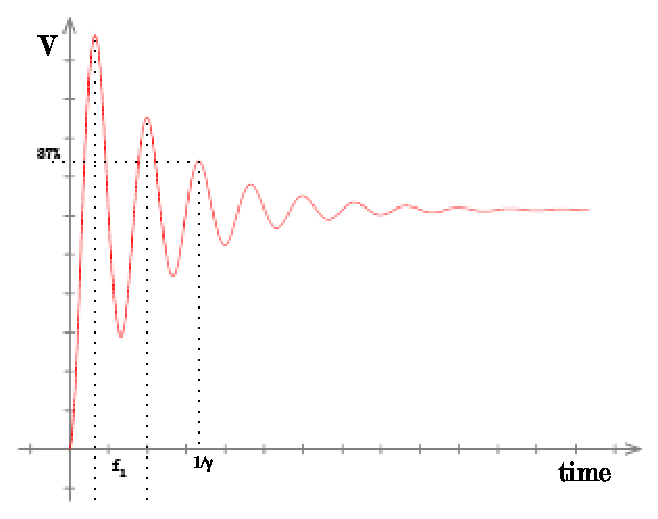
\includegraphics[scale=1.0]{DampOsc.eps}
\caption{\textit{The damped oscillator's response to a square wave input.}}
\label{DampOsc}
\end{figure}



\section{Experiment}
The general set up for all four circuits consisted of a bread board, function generator, and oscilloscope. The function generator's output voltage was connected to the first channel of the oscilloscope and to the breadboard. The trigger from the function generator was connected to channel 4 and the signal from the breadboard was fed into channel two. The connections from the signal generator were made with coaxial cables. The signal was connected by either a coaxial cable or the $10\times$ probe, which is used will be noted.

\subsection{The Voltage divider}
To begin we constructed the voltage divider circuit shown in figure \ref{FigVoltDiv} note that we connected the signal to the oscilloscope using a coaxial cable. Where $R_1=9.93\ k\Omega$ and $R_2=6.72 k\Omega$. We then sent a sinusoidal voltage into the circuit, with a voltage peak to peak of $V_{in} = 200\ mV\ P\ P$. We adjusted the oscilloscope so that the waveforms were clear on the screen we varied the frequency of the input voltage from $100\ Hz$ to $10\ MHz$ increasing a power of ten each step. Once we had the frequency set we used the cursors on the oscilloscope to measure the input voltage and the circuit's signal. Note that we placed each cursor at the peak of the waveform and recorded the difference. The recorded voltages are shown in table \ref{VoltDiv}.
\begin{table}[h]
\centering
\begin{tabular}{ccccc}
Frequency	&$V_{in}$	&$V_{out}$	&Attenuation($|T|$)	&Gain $dB$\\
\hline
$100\ Hz$	&$200\ mV$	&$84.0\ mV$	&$0.42$		&$-7.54\ dB$\\
$1.00\ kHz$	&$200\ mV$	&$80.0\ mV$	&$0.40$		&$-7.96\ dB$\\
$10.0\ kHz$	&$199\ mV$	&$80.0\ mV$	&$0.40$		&$-7.96\ dB$\\
$100\ kHz$	&$199\ mV$	&$78.0\ mV$	&$0.39$		&$-8.17\ dB$\\
$1.00\ MHz$	&$204\ mV$	&$39.0\ mV$	&$0.19$		&$-14.4\ dB$\\
$10.0\ MHz$	&$177\ mV$	&$4.0\ mV$	&$0.02$		&$-34.0\ dB$\\
\end{tabular}
\caption{\textit{The response of the voltage divider to varying frequencies. Note that attenuation and gain were calculated from equations \ref{atten} and \ref{gain}}}
\label{VoltDiv}
\end{table}

We see from equation \ref{VoltDiv.InvOut} that the transfer function is given by
$$\frac{V_{in}}{V_{out}} = \frac{R_2}{R_1+R_2}$$
Note that this is not dependent of frequency. So we expect the attenuation to be constant calculated as
$$\frac{6.72\ k\Omega}{9.93\ k\Omega+6.72\ k\Omega} = 0.404$$
We see that our data agrees with this expected attenuation except at high frequency. This is due to the capacitance in the coaxial cables, this effect is more pronounced at higher frequencies. This explains the drop in $|T|$ when the frequency exceeded $1\ MHz$. We see that a Bode plot (figure \ref{BodeVoltDivData}) of this data yields a flat line except at high frequency. 
\begin{figure}[h]
\centering
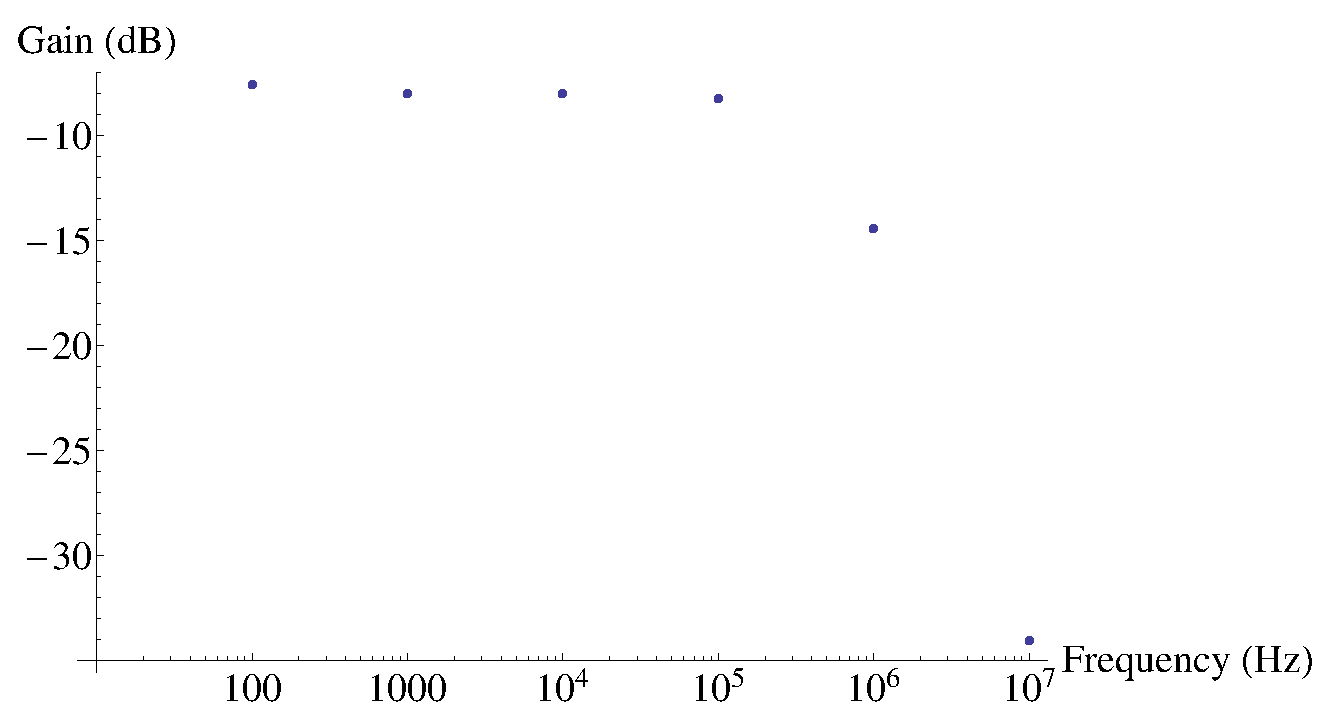
\includegraphics[scale=0.60]{BodeVoltDivData.eps}
\caption{\textit{The Bode plot of the data in table \ref{VoltDiv}}}
\label{BodeVoltDivData}
\end{figure}

Note we lost our original $R_2$ for all the parts that follow $R_2 = 6.69\ k\Omega$. Using equation \ref{VoltDiv.InvOut} we find that $|T| = 0.402$. Now are going to find the frequency at which the signal drops $3\ dB$. We know the output voltage stays constant at $124\ V$ so we want to find the frequency at which the output voltage is at $1/\sqrt{2}(124\ V) = 88.0\ V$. We adjusted the frequency until we found the voltage of our signal to be $88.0\ V$. We found this frequency to be $f_c = 715.4\ kHz$. We then repeated the process with the $10\times$ probe and found $f_c$ to be $1.00\ MHz$. So we see that the $10\times$ probe reduces the effect of the capacitance in the wire, but the effect is still not negligible.

Next we switched the input voltage from a sinusoidal wave to a square wave where the peak to peak voltage was $1\ V\ PP$. We note that the signal waveform is still a square wave with no exponential rise or decay. We then measure the input voltage and the signal voltage. We measured from the positive pulse to the negative pulse and found that $V_{in} = 2.04$ and $V_{out} = 0.920$. Calculating $|T|$ gives us $|T| = 0.45$ note that we expect $|T|$ to be $0.402$. This is a slight discrepancy is within reasonable bounds. 


\subsection{The Low-Pass Filter}
To start we constructed the circuit in figure \ref{FigLowPass} note that we connected the signal to the oscilloscope using a coaxial cable. Where $C = 1.001\ nF$ and $R = 9.93\ k\Omega$. Like the voltage divider we sent a sinusoidal voltage into the circuit, with a peak to peak voltage of $200\ mV\ PP$. We then varied the frequency of the input voltage from $10\ Hz$ to $10\ MHz$ increasing a power of ten in each step. We then measured the voltage in and the voltage out, these measurements are in table \ref{LowPass}.
\begin{table}[h]
\centering
\begin{tabular}{ccccc}
Frequency	&$V_{in}$	&$V_{out}$	&Attenuation($|T|$)	&$dB$\\
\hline
$10.0\ Hz$	&$206\ mV$	&$204\ mV$	&$0.99$		&$-0.087\ dB$\\
$100\ Hz$	&$206\ mV$	&$203\ mV$	&$0.99$		&$-0.087\ dB$\\
$1.00\ kHz$	&$206\ mV$	&$203\ mV$	&$0.99$		&$-0.087\ dB$\\
$10.0\ kHz$	&$206\ mV$	&$169\ mV$	&$0.82$		&$-1.72\ dB$\\
$100\ kHz$	&$204\ mV$	&$35.0\ mV$	&$0.17$		&$-15.4\ dB$\\
$1.00\ MHz$	&$202\ mV$	&$3.80\ mV$	&$0.019$	&$-34.4\ dB$\\
$10.0\ MHz$	&$178\ mV$	&$980\ \mu V$	&$0.006$	&$-44.4\ dB$\\
\end{tabular}
\caption{\textit{The response of the low-pass filter to varying frequencies. Note that attenuation and gain were calculated from equations \ref{atten} and \ref{gain}}}
\label{LowPass}
\end{table}

We see that the attenuation was near one for low frequencies but dropped quickly at higher frequencies. This is an expected reaction from the low-pass filter. We plot the data in table \ref{LowPass} in a Bode plot (see figure \ref{BodePlotLowPass}).
\begin{figure}[h]
\centering
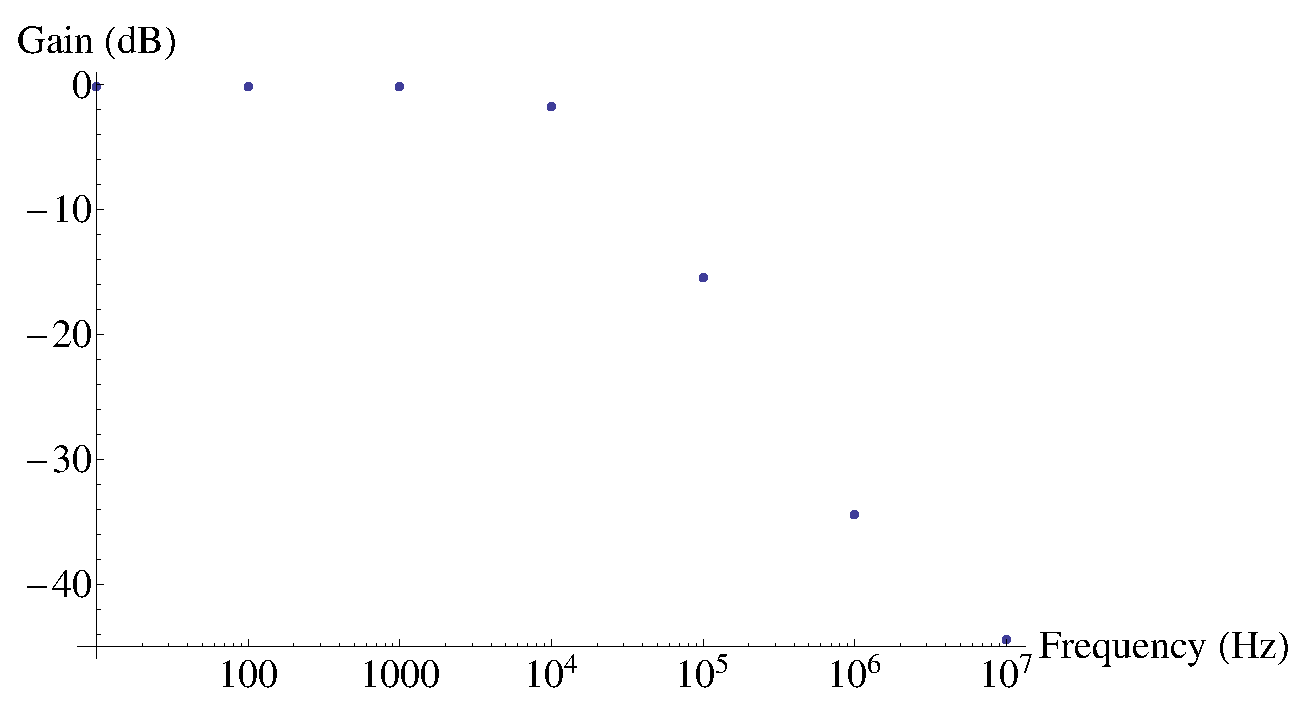
\includegraphics[scale=0.60]{BodePlotLowPass.eps}
\caption{\textit{The Bode plot of the data in table \ref{LowPass}}}
\label{BodePlotLowPass}
\end{figure}

Next we find the cut off frequency $f_c$ of the low pass filter. First we switch to the $10\times$ probe. Then we found the voltage in as $205\ mV$ and we found the voltage when $|T|$ drops $1/\sqrt{2}$ or the $3\ dB$ point. To find this voltage we calculated 
$$V_{out} = \frac{1}{\sqrt{2}}V_{in}$$
which we found as $V_{out} = 145\ mV$. So we adjusted the frequency until we reached this voltage difference in our signal. We found that $f_c = 18.9\ k\Omega$. Now from equation \ref{ResFreq} we can calculate the expected value of $f_c$ as
$$\frac{1}{2\pi(9.93\times10^{3}\ \Omega)(1.001\times10^{-6}\ F)} = 16.0\ kHz$$
We see that the measured result is about $20\%$ off of the expected value. This can be explained by the capacitance in the $10\times$ probe and the inaccuracy of the waveform on the oscilloscope.

Next we measured the phase difference of the signal with the input voltage at $0.1f_c$, $f_c$, and $10f_c$. We used the oscilloscopes phase measurement feature to find the phase difference in degrees. We adjusted the frequency to $0.1f_c$, $f_c$, and $10f_c$, then we recorded the phase change for each frequency (see table \ref{LowPassPhase}). Note that the measure function on the oscilloscope had a quickly changing measurement for the phase difference, so there is only one significant digit in this measurement.
\begin{table}[h]
\centering
\begin{tabular}{lcc}
		&Frequency	&Phase Change	\\
\hline
$0.1f_c$	&$1.36\ kHz$	&$2^{\circ}$\\
$f_c$		&$13.6\ kHz$	&$48^{\circ}$\\
$10f_c$		&$136\ kHz$	&$92^{\circ}$\\
\end{tabular}
\caption{\textit{The measured phase change of the low-pass filter at $0.1f_c$, $f_c$, and $10f_c$.}}
\label{LowPassPhase}
\end{table}
The data in table \ref{LowPassPhase} is plotted in figure \ref{PlotLowPassPhase}.
\begin{figure}[h]
\centering
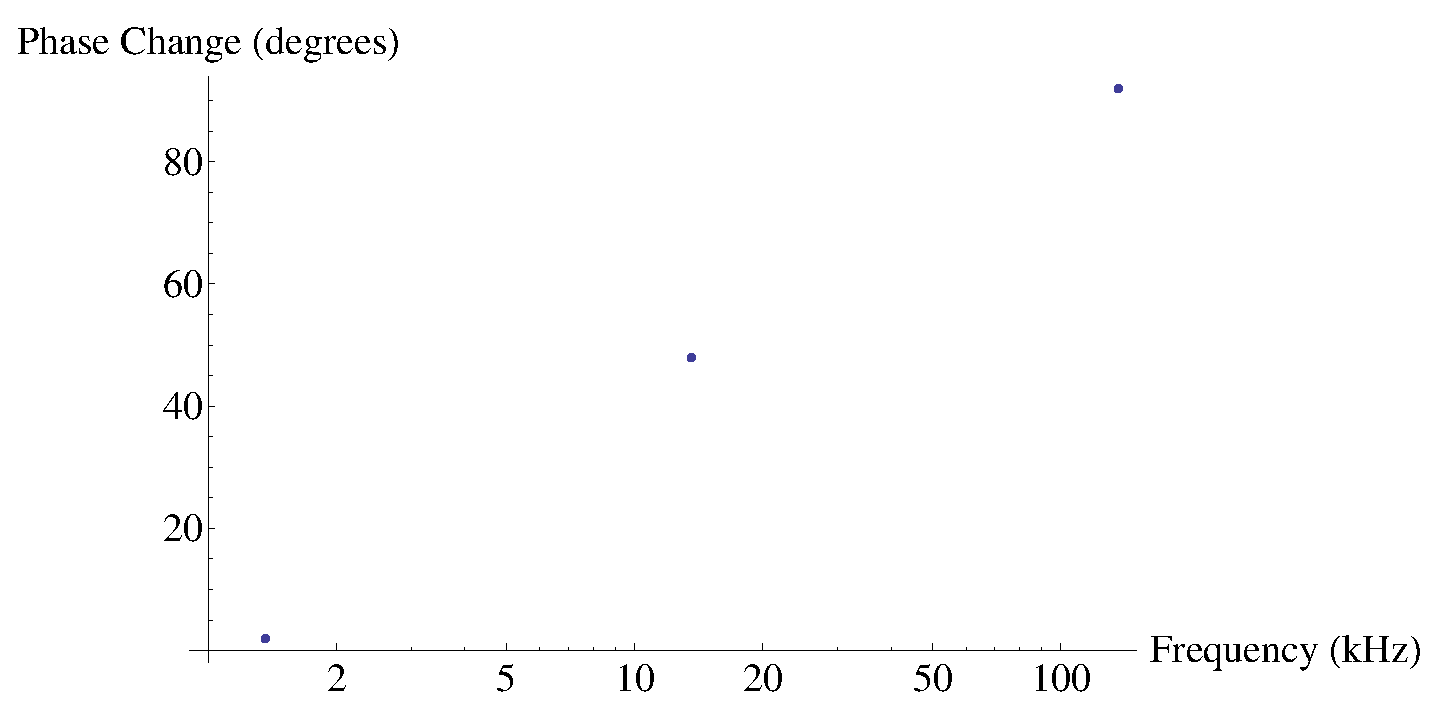
\includegraphics[scale=0.60]{PlotLowPassPhase.eps}
\caption{\textit{The phase plot of the data in table \ref{LowPassPhase}}}
\label{PlotLowPassPhase}
\end{figure}

Next we changed the input voltage to be a square wave with a voltage peak to peak of $1\ V\ PP$. Then we adjusted the frequency of the input voltage so that the exponential rise to fully rise before the next step in the square wave. Then we measured the maximum voltage of the signal as $1.02\ V$. Note that we measured from zero to the point where the waveform leveled off. Next we found the $67\%$ of the maximum voltage we found. We calculated this value as $(0.67)(1.02\ V) = 0.643\ V$. Now we measure the time it took for the wave form to rise from zero to $0.643\ V$, this value is the exponential rise time, $t_R$. We measured $t_R$ as $t_R =18.8\ \mu s$. We use equation \ref{TimeRise} to find the expected value of $t_R$ which we calculate as
$$t_R = (9.93\ k\Omega)(1.001\ nF) = 10.0 \mu s$$
We see that our measured exponential rise time is on the same order of our expected $t_R$.

\subsection{The High-Pass Filter}
To begin we made the circuit in figure \ref{FigHighPass} where $C=1.001\ nF$ and $R=9.93\ k\Omega$. Note that we used a coaxial cable to connect the signal to the oscilloscope. We adjusted our frequency from $100\ Hz$ to $10.0\ MHz$ in steps of that increased in powers of ten. We then measured and recorded the voltage in and the circuits signal (see table \ref{HighPass}).
\begin{table}[h]
\centering
\begin{tabular}{ccccc}
Frequency	&$V_{in}$	&$V_{out}$	&Attenuation($|T|$)	&$dB$\\
\hline
$100\ Hz$	&$205\ mV$	&$1.56\ mV$	&$0.008$	&$-41.9\ dB$\\
$1.00\ kHz$	&$204\ mV$	&$13.0\ mV$	&$0.063$	&$-24.0\ dB$\\
$10.0\ kHz$	&$205\ mV$	&$106\ mV$	&$0.517$	&$-5.73\ dB$\\
$100\ kHz$	&$204\ mV$	&$184\ mV$	&$0.902$	&$-0.896\ dB$\\
$1.00\ MHz$	&$202\ mV$	&$186\ mV$	&$0.921$	&$-0.715\ dB$\\
$10.0\ MHz$	&$156\ mV$	&$173\ mV$	&$1.11$		&$0.906\ dB$\\
\end{tabular}
\caption{\textit{The response of the high-pass filter to varying frequencies. Note that attenuation and gain were calculated from equations \ref{atten} and \ref{gain}}}
\label{HighPass}
\end{table}

We see that the high-pass filter had a high attenuation for high frequencies and low attenuation of low frequencies. This is the expected result. We plotted the data in table \ref{HighPass} in a Bode Plot (see figure \ref{BodePlotHighPass}).
\begin{figure}[h]
\centering
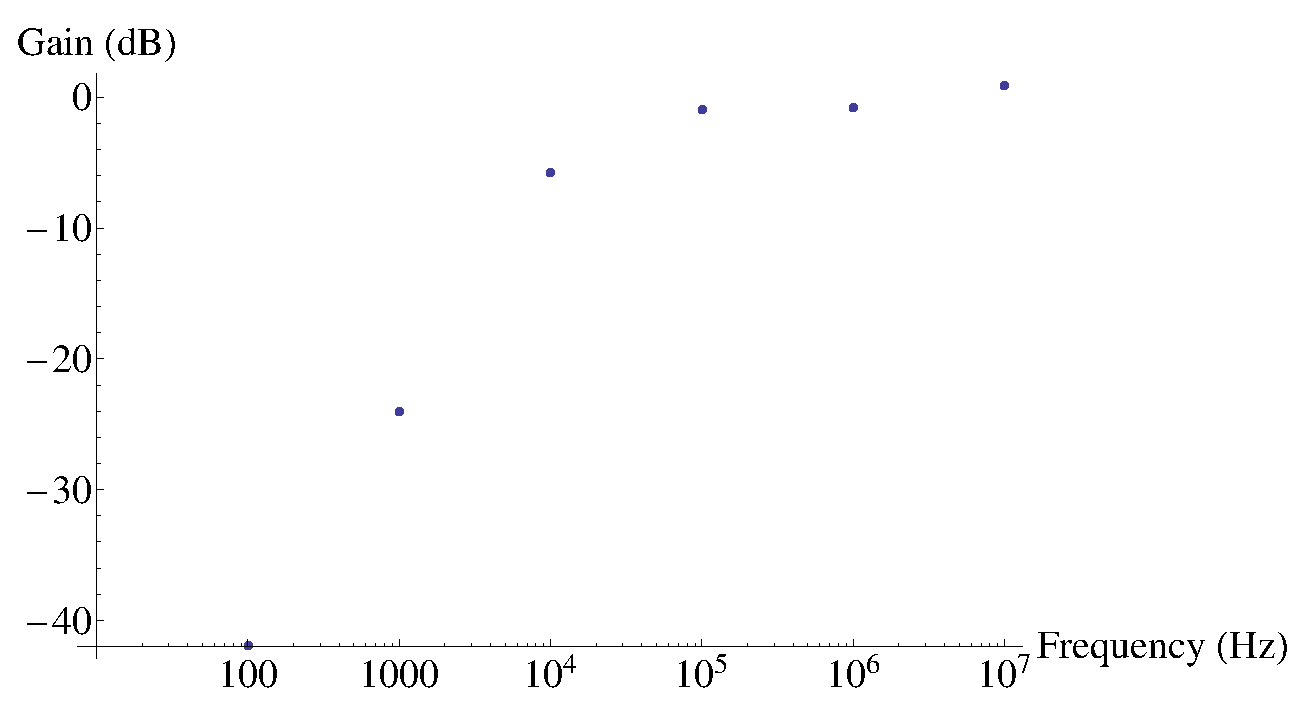
\includegraphics[scale=0.60]{BodePlotHighPass.eps}
\caption{\textit{The Bode plot of the data in table \ref{HighPass}}}
\label{BodePlotHighPass}
\end{figure}

Next we measure the cut off frequency $f_c$. First we used the $10\times$ probe to connect signal to the oscilloscope. Then we found that our voltage in was $204\ mV$ and we want to find the voltage out at the $3\ dB$ point so we calculated
$$V_{out} = \frac{1}{\sqrt{2}}(204\ mV) = 144\ mV$$
So we adjusted the frequency until we found that $V_{out} = 144$ we found that this point is $f_c = 13.6\ kHz$. Now we know from equation \ref{ResFreq} the expected resonant frequency is $16.0\ kHz$. Again we are off by about $20\%$, due to the capacitance in the $10\times$ probe and the uncertainty in the waveforms.

Next we measured the phase change of the signal from the input. We adjusted the frequency to $0.1f_c$, $f_c$, and $10f_c$ (note this is the $f_c$ we found experimentally) then used the measure function of the oscilloscope to find the phase difference in degrees and recorded the result (see table \ref{HighPassPhase}).
\begin{table}[h]
\centering
\begin{tabular}{lcc}
		&Frequency	&Phase Change	\\
\hline
$0.1f_c$	&$1.89\ kHz$	&$100^{\circ}$\\
$f_c$		&$18.9\ kHz$	&$50^{\circ}$\\
$10f_c$		&$189\ kHz$	&$8^{\circ}$\\
\end{tabular}
\caption{\textit{The measured phase change of the high-pass filter at $0.1f_c$, $f_c$, and $10f_c$.}}
\label{HighPassPhase}
\end{table}
The data from table \ref{HighPassPhase} was plotted (see figure \ref{PlotHighPassPhase}).
\begin{figure}[h]
\centering
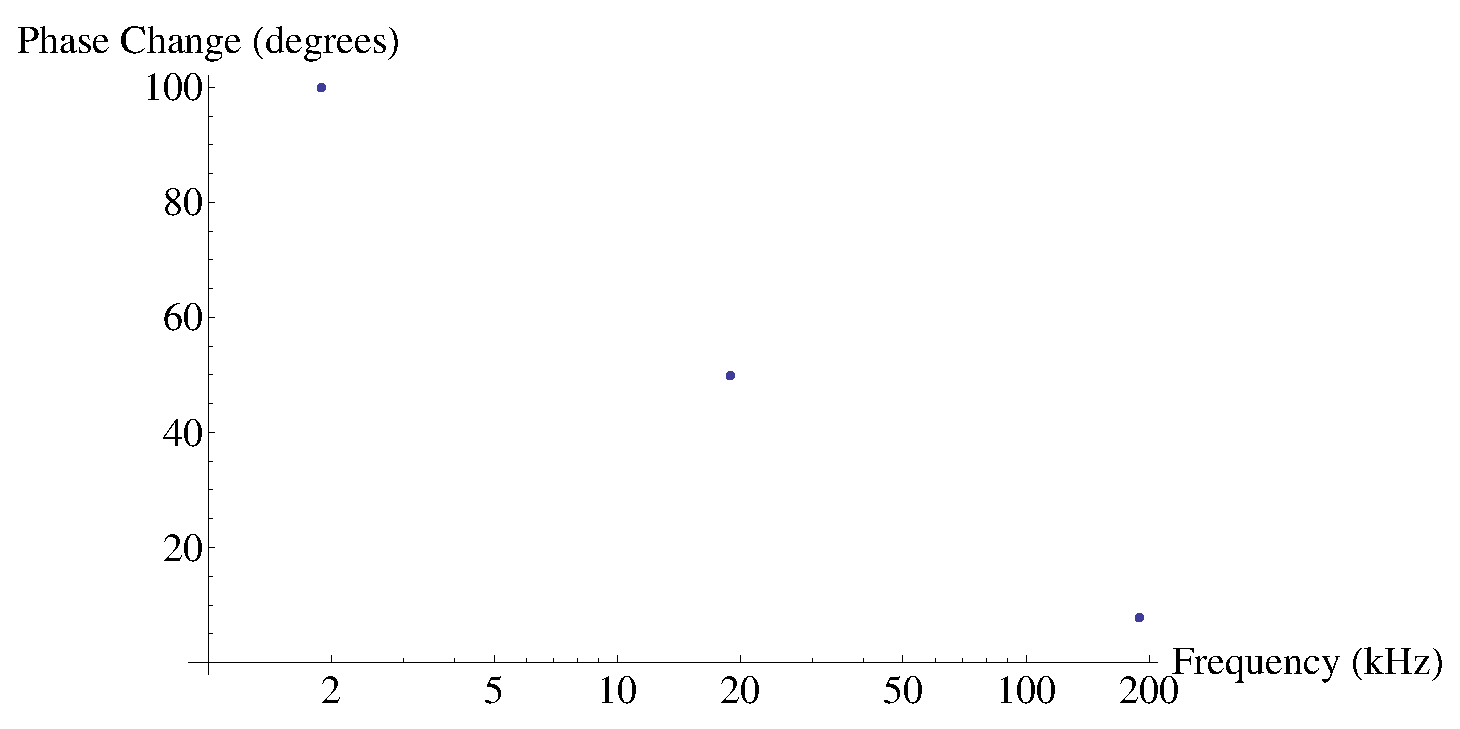
\includegraphics[scale=0.60]{PlotHighPassPhase.eps}
\caption{\textit{The phase plot of the data in table \ref{HighPassPhase}}}
\label{PlotHighPassPhase}
\end{figure}

Next we changed our input voltage to be in the form of a square wave with a voltage of $1\ V\ PP$. Note that we used the $10\times$ probe for this measurement. Next we adjusted the frequency of our input voltage so that the waveform of the signal could decay to $1\%$ of its final voltage before the next pulse in the square wave. Now we measured the maximum voltage of the signal. We found that $V_{max} = 1.01\ V$. Now we want to find the $37\%$ of the maximum voltage which we calculated to be $0.37\ V$. So we then found the time it took for the signal to decay to a voltage of $0.37\ V$. This time is the exponential time decay, $t_D$. We measured $t_D$ to be $18.2\ \mu s$. We can calculate the expected value of using equation \ref{TimeDecay} as $t_D = 10.0\ \mu s$. Like with the low-pass filter we are in the same order of magnitude with the expected result.

\subsection{The Band-Pass Filter}
To begin we created the circuit in figure \ref{FigBandPass} where $R=9.93$, $C=10.67\ nF$, and $L=11.09\ mH$. Note that we used the coaxial cable. We send a sinusoidal input voltage where the voltage of this wave is $1\ V\ PP$. Next we find the resonant frequency $f_0$ two ways. First we adjusted the frequency until we see that the voltage of the signal was at a maximum, once we reached that point we recorded the frequency. This method led us to $f_0 = 15.99\ kHz$. Next we adjusted the frequency until we found that the phases between the two lined up, and again we recorded this result. We found $f_0 = 15.96\ kHz$ using this method. We found that it was easier to match the phases then it was finding the maximum. So we will use $f_0 = 15.96\ kHz$ from here on out. Now we found the frequency at which out signal voltage dropped $3\ dB$. To do this we adjusted the frequency so that the signal peak to peak voltage was at $1.46\ V\ PP$. We found the lower frequency at this voltage to be $f_-=15.475\ kHz$ and the higher frequency to be $f_+ = 16.553$. Now we can find the bandwidth, $\Delta f$ of this circuit by taking the difference between these values. We found $\Delta f = 1.078\ kHz$. Now using equation \ref{QualDF} we can find the quality factor, $Q$, of this circuit as $Q = 15.96/1.078 = 14.8$. Now we can calculate the expected $Q$ from equation \ref{QualFact} 
$$Q = 2\pi(15.96\ kHz)(9.93\ k\Omega)(10.67\ nF) = 10.62$$
Note that the quality factor we measured is much higher than the $Q$ we expect. This is because we did not take into account the impedance of the oscilloscope.

Next we varied the frequency from $f_0-5\Delta f$ to $f_0+5\Delta f$ using steps that were multiples of $\Delta f$. For each frequency we measured the input voltage and the signal voltage and recorded the results (see table \ref{BandPass}).

\begin{table}[h]
\centering
\begin{tabular}{lccccc}
		&Frequency	&$V_{in}$	&$V_{out}$	&Attenuation($|T|$)	&$dB$\\
\hline
$f_0-5\Delta f$	&$10.57\ kHz$	&$2.05\ V$	&$0.252\ V$	&$0.123$		&$-18.2\ dB$\\
$f_0-2\Delta f$	&$13.80\ kHz$	&$2.05\ V$	&$0.690\ V$	&$0.337$		&$-9.45\ dB$\\
$f_0-\Delta f$	&$14.88\ kHz$	&$2.05\ V$	&$1.11\ V$	&$0.541$		&$-5.34\ dB$\\
$f_0-\Delta f/2$&$15.52\ kHz$	&$2.06\ V$	&$1.45\ V$	&$0.704$		&$-3.05\ dB$\\
$f_0-\Delta f/4$&$15.69\ kHz$	&$2.07\ V$	&$1.59\ V$	&$0.768$		&$-2.30\ dB$\\
$f_0$		&$15.96\ kHz$	&$2.07\ V$	&$1.66\ V$	&$0.802$		&$-1.92\ dB$\\
$f_0+\Delta f/4$&$16.23\ kHz$	&$2.07\ V$	&$1.63\ V$	&$0.787$		&$-2.08\ dB$\\
$f_0+\Delta f/2$&$16.50\ kHz$	&$2.06\ V$	&$1.51\ V$	&$0.733$		&$-2.70\ dB$\\
$f_0+\Delta f$	&$17.03\ kHz$	&$2.05\ V$	&$1.24\ V$	&$0.605$		&$-4.36\ dB$\\
$f_0+2\Delta f$	&$18.12\ kHz$	&$2.05\ V$	&$0.840\ V$	&$0.410$		&$-7.74\ dB$\\
$f_0+5\Delta f$	&$21.35\ kHz$	&$2.05\ V$	&$0.392\ V$	&$0.191$		&$-14.4\ dB$\\
\end{tabular}
\caption{\textit{The response of the band-pass filter to varying frequencies. Note that $f_0$ is the resonate frequency found from matching the phase of $V_{in}$ and $V_{out}$ and that $\Delta f$ was found by going $3\ dB$ down from $f_0$ and noting the frequency. The output voltage was measured using symmetric intervals around $f_0$. Note that attenuation and gain were calculated from equations \ref{atten} and \ref{gain}}}
\label{BandPass}
\end{table}

We see that the data in table \ref{BandPass} look Gaussian with a peak and a tail. This is what we expect from a band-pass filter. We plot the data in figure \ref{BodePlotBandPass}. 
\begin{figure}[h]
\centering
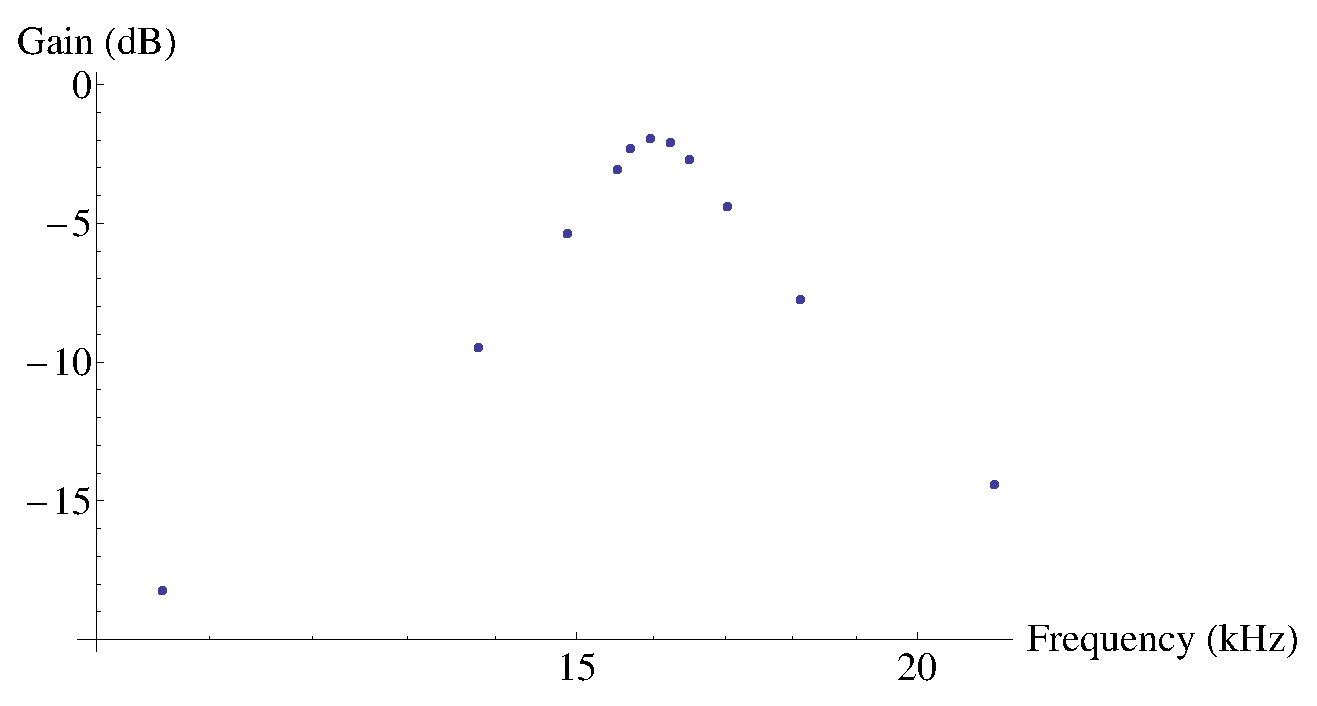
\includegraphics[scale=0.60]{BodePlotBandPass.eps}
\caption{\textit{The Bode plot of the data in table \ref{BandPass}}}
\label{BodePlotBandPass}
\end{figure}

Next we changed the voltage input from a sine wave to a square wave with a voltage of $1\ V\ PP$. Note that we used the $10\times$ probe for these measurements. Then we adjusted the frequency so that the signal waveform could decay to about $1\%$ of the maximum voltage before the next step in the square wave. Then we measured the period between the zero crossing of the signal. We used the zero crossing of the waveform rather than the peaks, because it was more accurate to find the zero crossings. We recorded five consecutive periods and the values we measured are in table \ref{BandPassPeriod}.
\begin{table}[h]
\centering
\begin{tabular}{lccccc}
	&Period($t_1$)		&Frequency($f_1$)\\
\hline
$1$	&$62.0\ \mu s$		&$16.13\ kHz$\\
$2$	&$62.0\ \mu s$		&$16.13\ kHz$\\
$3$	&$62.0\ \mu s$		&$16.13\ kHz$\\
$4$	&$62.0\ \mu s$		&$16.13\ kHz$\\
$5$	&$62.0\ \mu s$		&$16.13\ kHz$\\
\end{tabular}
\caption{\textit{The measured value for five consecutive periods of the damped oscillator. Note that $f_1=1/t_1$.}}
\label{BandPassPeriod}
\end{table}

Next we found that the first peak of the damped oscillator waveform was $V_{max}=180\ mV$. So we want to find the time it takes for the wave form to decay to $37\%$ of $V_{max}$ which we calculated as $70\ mV$. This time is the inverse of $\gamma$ or $1/\gamma$. We found $1/\gamma =122\ \mu s$ so we inverted this number and found that $\gamma = 8.20\ kHz$. Now we can find the quality factor using equation \ref{QualGamma}
$$Q = \frac{2\pi(15.96\ kHz)}{2(8.20\ kHz)} = 6.11$$
Note that we expected $Q=10.62$, but $\gamma$ was difficult to measure using the oscilloscope, as we had to switch between cursors. Some amount of ``eyeballing'' was used and explains this large discrepancy.

\section{Conclusion}
This lab experiment explained and demonstrated the properties of the low, high, and band-pass filters. We see that the names of these circuits are successful in describing how these circuits react to different frequencies. The low-pass filter filters out high frequencies and allows lower ones to pass. The high-pass filter filter out low frequencies and allows higher ones to pass. And the band-pass filter allows only a band of frequency to pass.

\end{document}

